\section{Thuật toán Colussi}

\subsection{Đặc điểm chính}
Thuật toán Colussi là một cải tiến của thuật toán Knuth-Morris-Pratt (KMP), được xây dựng dựa trên việc phân tích chặt chẽ cách KMP thực hiện so khớp và dịch chuyển mẫu. Thay vì quét các vị trí của mẫu theo thứ tự tuyến tính thông thường, Colussi chia tập vị trí của mẫu thành hai tập con rời nhau để tối ưu số phép so sánh ký tự.

Trong thuật toán này, một số vị trí của mẫu được quét từ trái sang phải, sau đó nếu không xảy ra mismatch thì các vị trí còn lại được quét từ phải sang trái. Cách tổ chức này giúp thuật toán tránh so sánh lại những ký tự đã biết chắc là khớp sau mỗi lần dịch chuyển.

Thuật toán có các đặc điểm sau:

\begin{itemize}
    \item là một cải tiến của thuật toán Knuth-Morris-Pratt;
    \item chia tập vị trí của mẫu thành hai tập con rời nhau;
    \item các vị trí trong tập thứ nhất được quét từ trái sang phải;
    \item nếu không xảy ra mismatch, các vị trí trong tập thứ hai được quét từ phải sang trái;
    \item giai đoạn tiền xử lý có độ phức tạp thời gian và không gian $O(m)$;
    \item giai đoạn tìm kiếm có độ phức tạp thời gian $O(n)$;
    \item trong trường hợp xấu nhất thực hiện không quá $\frac{3}{2}n$ phép so sánh ký tự văn bản.
\end{itemize}

\subsection{Mô tả thuật toán}
Việc thiết kế thuật toán Colussi dựa trên một phân tích chặt chẽ của thuật toán Knuth-Morris-Pratt.

Tập các vị trí của mẫu được chia thành hai tập con rời nhau. Khi đó, mỗi lần thử gồm hai giai đoạn:

\begin{itemize}
    \item trong giai đoạn thứ nhất, các phép so sánh được thực hiện từ trái sang phải với những ký tự văn bản được căn chỉnh với các vị trí của mẫu mà giá trị của hàm $\texttt{kmpNext}$ lớn hơn hẳn $-1$. Những vị trí này được gọi là \textbf{noholes};
    \item giai đoạn thứ hai thực hiện so sánh các vị trí còn lại, được gọi là \textbf{holes}, theo thứ tự từ phải sang trái.
\end{itemize}

Chiến lược này mang lại hai lợi ích:

\begin{itemize}
    \item khi xảy ra mismatch trong giai đoạn thứ nhất, sau khi thực hiện phép dịch chuyển thích hợp, không cần so sánh lại các ký tự văn bản đã được căn chỉnh với các vị trí noholes và đã được so sánh trong lần thử trước đó;
    \item khi xảy ra mismatch trong giai đoạn thứ hai, điều đó có nghĩa là một hậu tố của mẫu đã khớp với một đoạn của văn bản. Sau phép dịch chuyển tương ứng, một tiền tố của mẫu vẫn sẽ khớp với một đoạn của văn bản, do đó không cần so sánh lại đoạn này.
\end{itemize}

\textbf{Định nghĩa}

Với \(0 \leq i \leq m-1\), giá trị \(kmin[i]\) được định nghĩa như sau:

\[
kmin[i] =
\begin{cases}
d > 0, & \text{nếu } x[0 \ldots i-1-d] = x[d \ldots i-1] 
          \text{ và } x[i-d] \neq x[i], \\
0, & \text{ngược lại.}
\end{cases}
\]

Khi \(kmin[i] \neq 0\), ta nói rằng một tính chu kỳ kết thúc tại vị trí \(i\) trong mẫu \(x\).

Với \(0 < i < m\), vị trí \(i\) được phân loại như sau:

\[
i =
\begin{cases}
\text{nohole}, & \text{nếu } kmin[i-1] \neq 0, \\
\text{hole}, & \text{ngược lại.}
\end{cases}
\]

Gọi \(nd+1\) là số lượng vị trí \textbf{nohole} trong \(x\). Bảng \(h\) chứa trước tiên các vị trí \textbf{nohole} theo thứ tự tăng dần, sau đó chứa các vị trí \textbf{hole} theo thứ tự giảm dần:

\[
\begin{cases}
h[i] \text{ là nohole và } h[i] < h[i+1],
& 0 \leq i < nd, \\

h[i] \text{ là hole và } h[i] > h[i+1],
& nd < i < m-1.
\end{cases}
\]

Nếu \(i\) là một \textbf{hole}, thì \(rmin[i]\) là chu kỳ nhỏ nhất của \(x\) lớn hơn \(i\). Giá trị \(first[u]\) là số nguyên nhỏ nhất \(v\) sao cho:

\[
first[u] = \min \{\, v \mid u \leq h[v] \,\}.
\]

Giả sử mẫu \(x\) được căn chỉnh với đoạn văn bản \(y[j \ldots j+m-1]\).

Nếu trong giai đoạn so sánh các vị trí \textbf{nohole} ta có:

\[
x[h[k]] = y[j+h[k]], \quad 0 \leq k < r < nd
\]

và xảy ra mismatch tại vị trí \(h[r]\):

\[
x[h[r]] \neq y[j+h[r]],
\]

thì đặt:

\[
j' = j + kmin[h[r]].
\]

Khi đó không tồn tại lần xuất hiện nào của \(x\) bắt đầu trong đoạn \(y[j \ldots j']\), nên mẫu có thể được dịch sang phải \(kmin[h[r]]\) vị trí. Hơn nữa:

\[
x[h[k]] = y[j' + h[k]],
\quad
0 \leq k < first[h[r] - kmin[h[r]]].
\]

Do đó, quá trình so sánh có thể được tiếp tục từ:

\[
x[h[first[h[r] - kmin[h[r]]]]]
\quad \text{và} \quad
y[j' + h[first[h[r] - kmin[h[r]]]]].
\]

\begin{figure}[H]
    \centering
    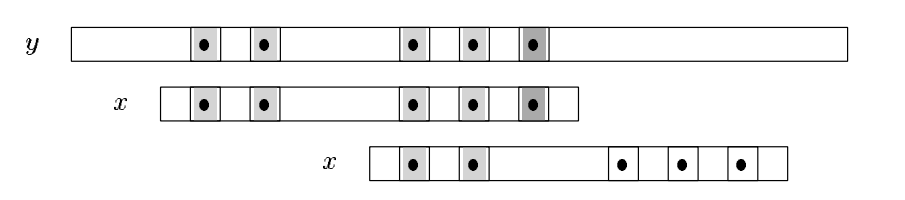
\includegraphics[width=15cm]{Images/2026-05-18-14-04-48.png}
    \label{fig:colussi-nohole-shift}
\end{figure}

Nếu trong giai đoạn so sánh các vị trí \textbf{hole} ta có:

\[
x[h[k]] = y[j+h[k]], \quad 0 \leq k < r
\]

và xảy ra mismatch tại vị trí \(h[r]\), với \(nd \leq r < m\):

\[
x[h[r]] \neq y[j+h[r]],
\]

thì đặt:

\[
j' = j + rmin[h[r]].
\]

Khi đó không tồn tại lần xuất hiện nào của \(x\) bắt đầu trong đoạn \(y[j \ldots j']\), nên mẫu có thể được dịch sang phải \(rmin[h[r]]\) vị trí. Hơn nữa:

\[
x[0 \ldots m-1-rmin[h[r]]]
=
y[j' \ldots j+m-1].
\]

Do đó, quá trình so sánh có thể được tiếp tục từ:

\[
x[h[first[m-1-rmin[h[r]]]]]
\quad \text{và} \quad
y[j' + h[first[m-1-rmin[h[r]]]]].
\]

\begin{center}
    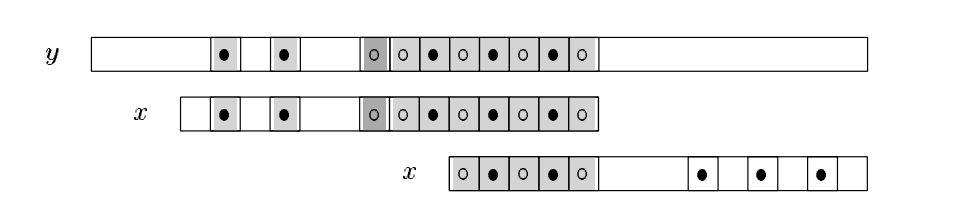
\includegraphics[width=15cm]{Images/2026-05-18-14-07-41.png}
\end{center}

Trong tình huống này, sau khi dịch chuyển, thuật toán không cần so sánh lại phần tiền tố đã khớp của mẫu.

Để tính các giá trị của \(kmin\), thuật toán sử dụng bảng \(hmax\), được định nghĩa như sau: \(hmax[k]\) là giá trị thỏa mãn

\[
x[k \ldots hmax[k]-1]
=
x[0 \ldots hmax[k]-k-1]
\]

và

\[
x[hmax[k]] \neq x[hmax[k]-k].
\]

Giá trị \(nhd0[i]\) là số lượng vị trí \textbf{nohole} nhỏ hơn hẳn \(i\).

Ta có thể định nghĩa hai hàm \(shift\) và \(next\) như sau:

\[
shift[i] =
\begin{cases}
kmin[h[i]], & i < nd, \\
rmin[h[i]], & nd \leq i < m, \\
rmin[0], & i = m,
\end{cases}
\]

\[
next[i] =
\begin{cases}
nhd0[h[i]-kmin[h[i]]], & i < nd, \\
nhd0[m-rmin[h[i]]], & nd \leq i < m, \\
nhd0[m-rmin[h[m-1]]], & i = m.
\end{cases}
\]

Do đó, trong một lần thử khi cửa sổ được đặt trên đoạn văn bản \(y[j \ldots j+m-1]\), nếu xảy ra mismatch giữa \(x[h[r]]\) và \(y[j+h[r]]\), thì cửa sổ cần được dịch sang phải một đoạn bằng:

\[
shift[r].
\]

Sau đó, quá trình so sánh có thể được tiếp tục từ vị trí mẫu:

\[
h[next[r]].
\]

Giai đoạn tiền xử lý có thể được thực hiện với độ phức tạp thời gian và không gian \(O(m)\). Giai đoạn tìm kiếm có độ phức tạp thời gian \(O(n)\). Hơn nữa, trong giai đoạn tìm kiếm, thuật toán thực hiện không quá \(\frac{3}{2}n\) phép so sánh ký tự của văn bản.

\subsection{Cài đặt bằng C++}

\begin{verbatim}
#include <iostream>
#include <vector>
#include <string>

using namespace std;

/* ---------- Preprocessing for Colussi ---------- */
int preColussi(const string &pat,
               vector<int> &h,
               vector<int> &next,
               vector<int> &shift) {
    int m = pat.length();

    int i, k, nd, q, r, s;

    vector<int> hmax(m + 1, 0);
    vector<int> kmin(m + 1, 0);
    vector<int> nhd0(m + 1, 0);
    vector<int> rmin(m + 1, 0);

    h.assign(m + 1, 0);
    next.assign(m + 1, 0);
    shift.assign(m + 1, 0);

    /* Computation of hmax */
    i = k = 1;

    do {
        while (i < m && pat[i] == pat[i - k]) {
            ++i;
        }

        hmax[k] = i;

        q = k + 1;

        while (q <= m && hmax[q - k] + k < i) {
            hmax[q] = hmax[q - k] + k;
            ++q;
        }

        k = q;

        if (k == i + 1) {
            i = k;
        }

    } while (k <= m);

    /* Computation of kmin */
    for (i = 0; i < m; ++i) {
        kmin[i] = 0;
    }

    for (i = m; i >= 1; --i) {
        if (hmax[i] < m) {
            kmin[hmax[i]] = i;
        }
    }

    /* Computation of rmin */
    r = 0;

    for (i = m - 1; i >= 0; --i) {
        if (hmax[i + 1] == m) {
            r = i + 1;
        }

        if (kmin[i] == 0) {
            rmin[i] = r;
        } else {
            rmin[i] = 0;
        }
    }

    /* Computation of h */
    s = -1;
    r = m;

    for (i = 0; i < m; ++i) {
        if (kmin[i] == 0) {
            h[--r] = i;
        } else {
            h[++s] = i;
        }
    }

    nd = s;

    /* Computation of shift */
    for (i = 0; i <= nd; ++i) {
        shift[i] = kmin[h[i]];
    }

    for (i = nd + 1; i < m; ++i) {
        shift[i] = rmin[h[i]];
    }

    shift[m] = rmin[0];

    /* Computation of nhd0 */
    s = 0;

    for (i = 0; i < m; ++i) {
        nhd0[i] = s;

        if (kmin[i] > 0) {
            ++s;
        }
    }

    /* Computation of next */
    for (i = 0; i <= nd; ++i) {
        next[i] = nhd0[h[i] - kmin[h[i]]];
    }

    for (i = nd + 1; i < m; ++i) {
        next[i] = nhd0[m - rmin[h[i]]];
    }

    next[m] = nhd0[m - rmin[h[m - 1]]];

    return nd;
}

/* ---------- Colussi Algorithm ---------- */
void Colussi(const string &pat, const string &txt) {
    int m = pat.length();
    int n = txt.length();

    if (m == 0 || n < m) {
        return;
    }

    vector<int> h;
    vector<int> next;
    vector<int> shift;

    /* Preprocessing */
    int nd = preColussi(pat, h, next, shift);

    /* Searching */
    int i = 0;
    int j = 0;
    int last = -1;

    while (j <= n - m) {
        while (i < m &&
               last < j + h[i] &&
               pat[h[i]] == txt[j + h[i]]) {
            ++i;
        }

        if (i >= m || last >= j + h[i]) {
            cout << "Pattern found at index: " << j << endl;
            i = m;
        }

        if (i > nd) {
            last = j + m - 1;
        }

        j += shift[i];
        i = next[i];
    }
}

/* ---------- Main ---------- */
int main() {
    string text = "ABAAABCDABCABC";
    string pattern = "ABC";

    Colussi(pattern, text);

    return 0;
}
\end{verbatim}

\subsection{Kiểm nghiệm thuật toán}
\textbf{Pha tiền xử lý:}

\begin{center}
    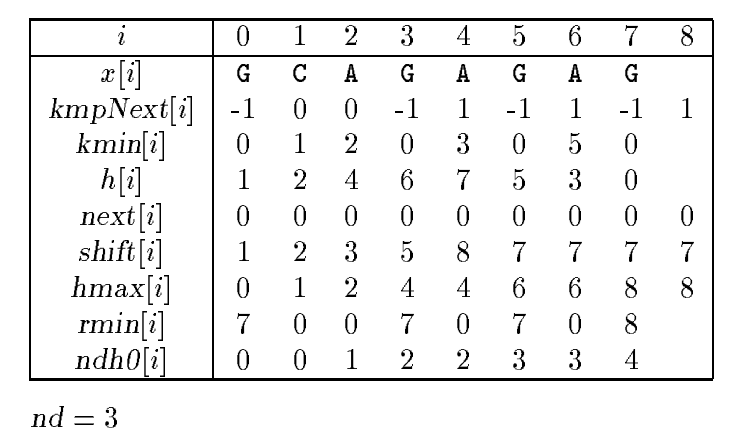
\includegraphics[width=15cm]{Images/2026-05-18-14-11-22.png}
\end{center}

Bảng được sử dụng bởi thuật toán Colussi.

\textbf{Pha tìm kiếm:}

Lần 1:

\begin{center}
    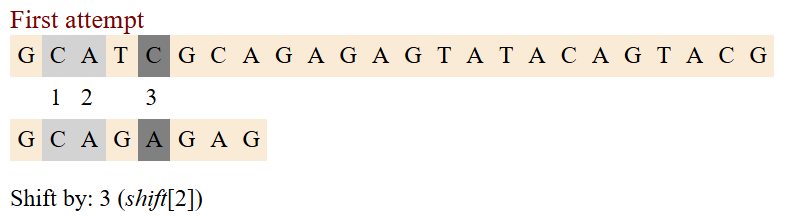
\includegraphics[width=15cm]{Images/2026-05-18-14-12-49.png}
\end{center}
Lần 2:

\begin{center}
    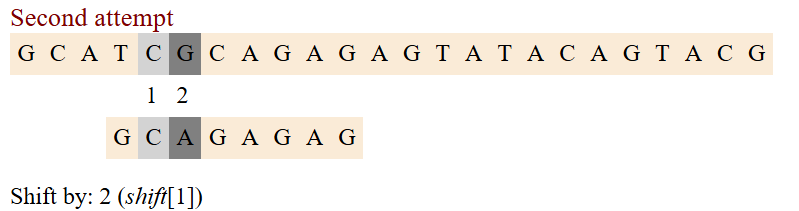
\includegraphics[width=15cm]{Images/2026-05-18-14-12-56.png}
\end{center}
Lần 3:

\begin{center}
    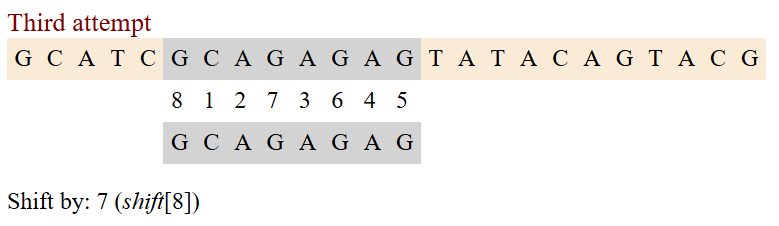
\includegraphics[width=15cm]{Images/2026-05-18-14-13-05.png}
\end{center}
Lần 4:

\begin{center}
    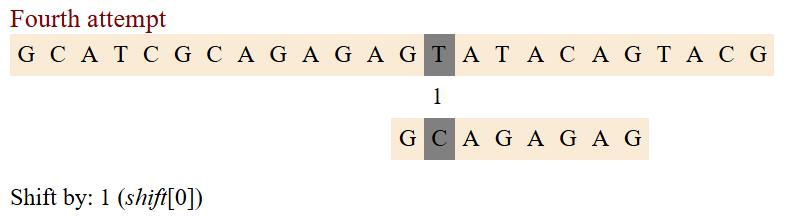
\includegraphics[width=15cm]{Images/2026-05-18-14-13-14.png}
\end{center}
Lần 5:

\begin{center}
    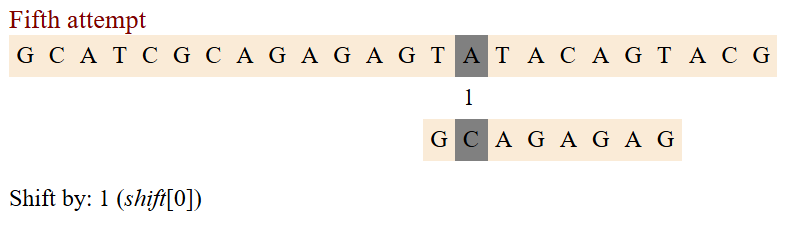
\includegraphics[width=15cm]{Images/2026-05-18-14-13-22.png}
\end{center}
Lần 6:

\begin{center}
    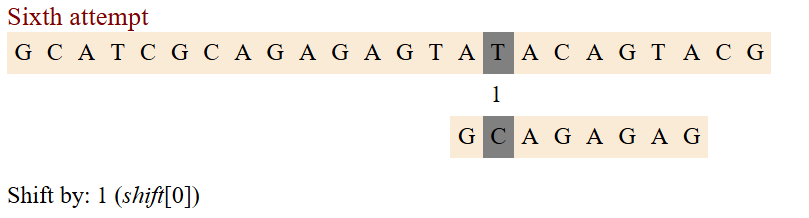
\includegraphics[width=15cm]{Images/2026-05-18-14-13-33.png}
\end{center}
Lần 7:

\begin{center}
    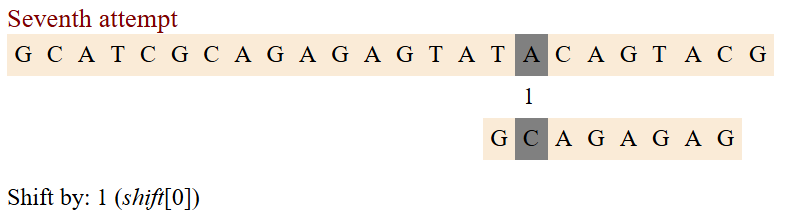
\includegraphics[width=15cm]{Images/2026-05-18-14-13-41.png}
\end{center}
Lần 8:

\begin{center}
    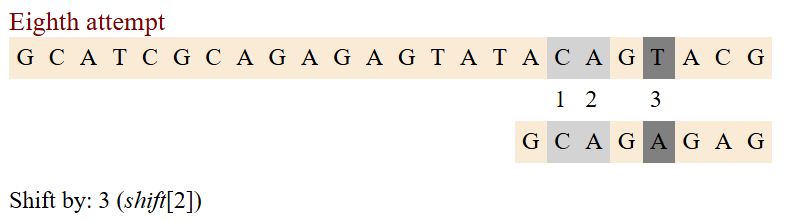
\includegraphics[width=15cm]{Images/2026-05-18-14-13-49.png}
\end{center}

Thuật toán Colussi thực hiện 20 lần so sánh ký tự trong ví dụ trên.